\subsection{Analysis of the DCM}

\subsubsection{Model selection}
In order to choose  parsimonious models with good performance, two different types of models are considered, namely, Full models, which contain all \num{12} covariates (weather, distances, lockdown, holiday) assigned to $x_{\beta}$, whereas initially only the constant was assigned to $x_{z}$, and Selected models, which include only those covariates that are significant.
The model selection was carried out on the univariate spatio-temporal process related to pickups, on the univariate spatio-process process related to the average trip duration and on the bivariate spatio-temporal process (pickup, trip duration). 
The model selection for each model consists in evaluating at each iteration, in removing the coviariate least significance until the model reaches a significance level of \num{5}\%. 
In the selected model, after model selection on $x_{\beta}$, it was also done on $x_{z}$ by using a forward approach (on spatial and dummy covariates), and choosing the model with the lowest $rmse_{s}$ among those tested.
After obtaining the various models, have been evaluated their performance in comparison to the full models and their predictive ability through the Cross Validation (table \ref{Cross-validation rmse_s DCM}). 
The table \ref{Model_selection_pickups} shows the model selection related to the univariate process of the pickups,  after being performed on the $x_{\beta}$, it was performed on the coefficients of the latent variable $x_{z}$ and it resulted that with only the constant the lowest  $rmse_{s}$  is obtained.




 \begin{table}[h!]
	\centering
	\renewcommand\arraystretch{1.3}
	\begin{tabular}{c|c|c|c}
		\hline
		\textit{} & \textit{Number of}  &  &    \\
		\textit{Step} & \textit{regressor in the}  & Least significant & p-value \\
		\textit{Model} & \textit{model}  & regressor &  \\
		\hline
		\textbf{1} & \num{12} & visibility & \num{48.40}\%  \\
		\hline
		\textbf{2} & \num{11} & holiday & \num{48.05}\%  \\
		\hline
		\textbf{3} & \num{10} & snowfall & \num{45.11}\%  \\
		\hline
		\textbf{4} & \num{9} & humidity & \num{38.17}\%  \\
		\hline
		\textbf{5} & \num{8} & windspeed & \num{6.11}\% \\
		\hline
		\textbf{6} & \num{7} & cloud cover & \num{10.37}\%  \\
		\hline
		\textbf{7} & \num{6} & /  &  / \\
		\hline
	\end{tabular}
	\caption[Model selection on the univariate process related to pickups (DCM).]{Model selection on the univariate process related to pickups (DCM).}
	\label{Model_selection_pickups}
\end{table}
\noindent


The same procedure was performed on the average trip duration and on the bivariate case, the best model for the trip duration that has been achieved has \num{6} covariates assigned to $x_{\beta}$ and \num{3} covariates (constant,distance,lockdown) assigned to $x_{z}$,
while for the bivariate case \num{12} covariates were assigned to $x_{\beta}$  and \num{4} (constant,distance for both process) to $x_{z}$. 
The table \ref{beta coefficients} shows the values of the estimated $\beta$ coefficients and their assignments.






\subsubsection{Model analysis}

The table \ref{beta coefficients} shows the beta coefficients estimated after performing the model selection, and it can be osserve that the most significant covariate for each process is the temperature. The only difference between the pickups and trip duration processes is that the covariate holiday is not considered in the pickups processes, while for the average trip duration the lockdown is not considered.
 \begin{table}[h!]
	\centering
	\renewcommand\arraystretch{1.3}
	\begin{tabular}{c|c|c|c|c|c|c|c}
		\hline
		\textit{} & $\boldsymbol{\hat{\beta}_{const}}$  & $\boldsymbol{\hat{\beta}_{temp}}$ & $\boldsymbol{\hat{\beta}_{rain}}$ & $\boldsymbol{\hat{\beta}_{dist}}$ & $\boldsymbol{\hat{\beta}_{Holiday}}$ & $\boldsymbol{\hat{\beta}_{Lock}}$ & $\boldsymbol{\hat{\beta}_{UV}}$ \\
		\hline
		\textbf{2-variate} & {\fontsize{3mm}{4mm}$+0.017_{(0.118)}$} & {\fontsize{3mm}{4mm}$+0.293_{(0.149)}$}  & {\fontsize{3mm}{4mm}$-0.060_{(0.021)}$} &	 {\fontsize{3mm}{4mm}$-0.137_{(0.009)}$} &  & {\fontsize{3mm}{4mm}$-0.586_{(0.148)}$} & {\fontsize{3mm}{4mm}$+0.172_{(0.029)}$}  \\
		\textbf{Pickups} & &  &  & & & &  \\
		\hline
		\textbf{2-variate} & {\fontsize{3mm}{4mm}$-0.041_{(0.186)}$} & {\fontsize{3mm}{4mm}$+0.272_{(0.040)}$}  & {\fontsize{3mm}{4mm}$-0.031_{(0.040)}$} &	 {\fontsize{3mm}{4mm}$-0.099_{(0.009)}$} & {\fontsize{3mm}{4mm}$+229_{(0.039)}$} &  & {\fontsize{3mm}{4mm}$+0.138_{(0.02)}$}  \\
		\textbf{Duration} &  & & & & & &  \\
		\hline
		\textbf{1-variate}  &{\fontsize{3mm}{4mm}$+0.065_{(0.153)}$} & {\fontsize{3mm}{4mm}$+0.274_{(0.052)}$}  & {\fontsize{3mm}{4mm}$-0.056_{(0.030)}$} &	 {\fontsize{3mm}{4mm}$-0.136_{(0.009)}$} &  & {\fontsize{3mm}{4mm}$-0.690_{(0.156)}$} & {\fontsize{3mm}{4mm}$+0.123_{(0.039)}$}  \\
		\textbf{Pickups} & & & & & & &  \\
		\hline
		\textbf{1-variate} & {\fontsize{3mm}{4mm}$-0.050_{(0.173)}$} & {\fontsize{3mm}{4mm}$+0.282_{(0.036)}$}  & {\fontsize{3mm}{4mm}$-0.030_{(0.013)}$} &	 {\fontsize{3mm}{4mm}$-0.104_{(0.010)}$} & {\fontsize{3mm}{4mm}$+0.229_{(0.037)}$}  &  & {\fontsize{3mm}{4mm}$+0.139_{(0.018)}$}  \\
		\textbf{Duration} &  &  &  & & & &  \\
		\hline

	\end{tabular}
	\caption[Estimated $\boldsymbol{\beta}$ for the bivariate model and 1-variate models (DCM).]{Estimated $\boldsymbol{\beta}$ for the bivariate model and 1-variate models (DCM).}
	\label{beta coefficients}
\end{table}
\noindent

Figure \ref{Trend_zeta_latente univariato} explain the trend of the latent z(t) of the average trip duration interacting with the covariates:
\begin{itemize}
	\item $z_{1,constant}$, which indicates the trend of the average trip duration, during the first months of the year, the average duration of trips is below average, while with the arrival of the lockdown there is a significant increase in the average duration of trips until the end of the year.
	\item $z_{2,distance}$, which indicates the distance. the trend for the whole year does not have much influence
	\item $z_{3,Holidays}$ , which related to the holidays, and not affect the increase of trip duration.
\end{itemize}
\noindent


\begin{figure}[h!]
	\centering
	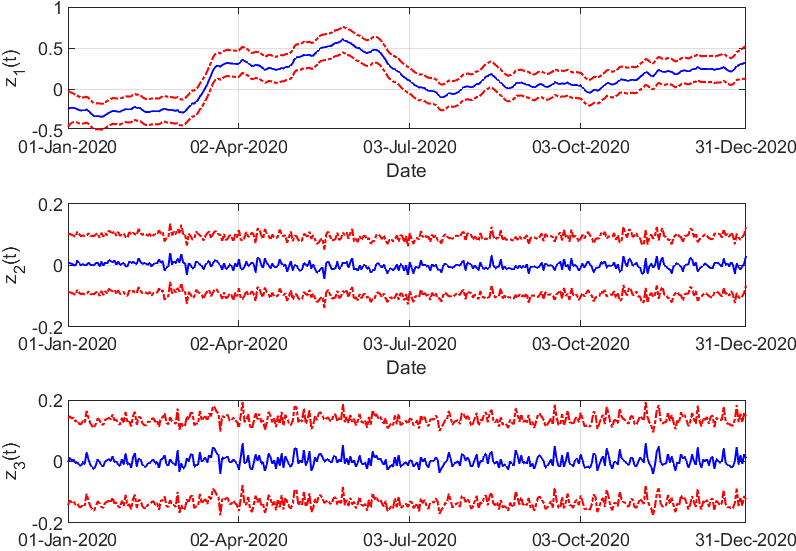
\includegraphics[height=250px]{Images/Data analysis/DCM/trend_z_selected_trip_model.png}
	\caption[Estimated $z_{1}(t)$,  $z_{2}(t)$ and $z_{3}(t)$ by Kalman smoother in the univariate model for pickups (DCM)]{Estimated $z_{1,constant}(t)$,  $z_{2,distance}(t)$ and $z_{3,Holidays}(t)$ by Kalman smoother in the univariate model for the average trip duration.}
	\label{Trend_zeta_latente univariato}
	
\end{figure}

\noindent
Figure \ref{Trend_zeta_latente_biv} shows the trend of the latent z interacting with the covariates:
\begin{itemize}
	\item $z_{1,constant,pick}$, which indicates the trend of the pickups, and it is noted that the trend of pickups is below the average except for the first three months of the year and for some days at the end of October where there is a small one which could be due to the closure of the metro
	\item $z_{2,distance,pick}$, is refers to the distance. it is noted that throughout the year it brings a decrease in pickups
	\item $z_{3,constant,duration}$ , which indicates the trend of the average of trip duration, it's very similar to the univariate case.
	\item $z_{4,constant,pick}$ , which is relatite to the distance, and not affect the increase of the average trip duration.
\end{itemize}

\begin{figure}[h!]
	\centering
	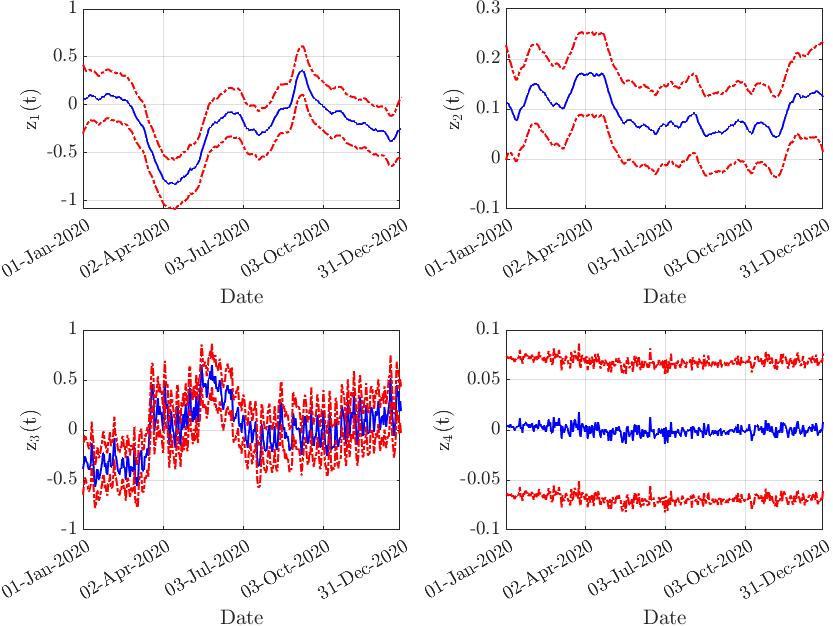
\includegraphics[height=300px]{Images/Data analysis/DCM/trend_z_bivariate_selected_DCM.png}
	\caption[Estimated $z_{1,constant,pick}(t)$,  $z_{2,distance,pick}(t)$ , $z_{3,constant,duration}(t)$ and $z_{4,distance,duration}(t)$ by Kalman smoother in the bivariate model (DCM)]{Estimated $z_{1,constant,pickups}(t)$,  $z_{2}(t)$ and $z_{3}(t)$ by Kalman smoother in the bivariate model (DCM)}
	\label{Trend_zeta_latente_biv}
\end{figure}
\noindent

The table \ref{Cross-validation rmse_s DCM} illustrate the different $rmse_{s}$ obtained from the models, and it is noted that there is a lot of difference both between the univariate cases and the bivariate case and between the complete models and the selected ones. For the daily rental duration, the selected univariate model is the best.

\begin{table}[h!]
	\centering
	\renewcommand\arraystretch{1.3}
	\begin{tabular}{c|cc|cc}
		\hline
		\multicolumn{1}{l|}{} & \multicolumn{2}{c|}{\textit{CV $RMSE_{s}$, full model}} & \multicolumn{2}{c}{\textit{CV MSE, selected model} }\\ 
		\hline
		\textit{Model} & \multicolumn{1}{c|}{\textit{Pickups}} & \textit{Trip duration} & \multicolumn{1}{c|}{\textit{Pickups}} & \textit{Trip duration} \\ 
		\hline
		\textbf{2-variate } & \multicolumn{1}{c|}{0.6045}  & 0.8403   & \multicolumn{1}{c|}{0.6042}  & 0.8403   \\ 
		\hline
		\textbf{1-variate } & \multicolumn{1}{c|}{0.6032}  & 0.8403   & \multicolumn{1}{c|}{0.6033}  & 0.8400   \\ 
		\hline
	\end{tabular}
	\caption[RMSE concerning cross-validation in log-standardized scale for response variables, (DCM))]{RMSE concerning cross-validation in log-standardized scale for response variables, (DCM).}
	\label{Cross-validation rmse_s DCM}
\end{table}